%%%%%%%%%%%%%%%%%%%%%%%%%%%%%%%%%%%%%%%%%%%%%%%%%%%%%%%%%%%%%%%%%%%%%%%%%%%%%%%%%%
\begin{frame}[fragile]\frametitle{}
\begin{center}
{\Large Introduction to Patanjali Yog-Sutra}
\end{center}
\end{frame}

%%%%%%%%%%%%%%%%%%%%%%%%%%%%%%%%%%%%%%%%%%%%%%%%%%%%%%%%%%%
 \begin{frame}[fragile]\frametitle{Patanjali  पतञ्जलि }
 
    \begin{columns}
    \begin{column}[t]{0.4\linewidth}
	
\begin{center}
\includegraphics[width=0.5\linewidth,keepaspectratio]{images/yog15}
\end{center}

\begin{sanskrit}
योगेन चित्तस्य पदेन वाचां |
मलं शरीरस्य च वैद्यकेन |
योऽपाकरोक्तं प्रवरं मुनीनां |
पतञ्जलिं प्राञ्जलिरनतोस्मि ||
- राजा भर्तुहरि
\end{sanskrit}

    \end{column}
    \begin{column}[t]{0.6\linewidth}
		\begin{itemize}
	\item Patajali has been mentioned to have 3 contributions (two of them are lost in time)
	\item चित्तशुद्धि Purification of mind using Yog
	\item Purification of speech using Grammar
	\item Purification of body using medicine (Ayurveda)
	\item Better amongst sages, we salute Rishi Patanjali
	\end{itemize}

    \end{column}
  \end{columns}
\end{frame}

%%%%%%%%%%%%%%%%%%%%%%%%%%%%%%%%%%%%%%%%%%%%%%%%%%%%%%%%%%%
\begin{frame}[fragile]\frametitle{Maharshi Patanjali महर्षि पतञ्जलि}

	\begin{itemize}
	\item Considered as `the father of Yoga'.
\item Many believe he’s thought to have lived between 200 and 500 B.C. 
\item At the time when the Ayurveda was the greatest wisdom, people had to cure their illness.	
\item Since, being sick it is not just sickness in the body, but also the sickness in the mind and emotions. 
\item The Yoga Sutras of Patanjali projects the knowledge that doesn’t just cure the body but also purify the mind, emotions and the complete existence itself, all through Yoga.
	\end{itemize}

\tiny{(Ref: Basic Introduction of Patanjali Yoga Sutras – The Best Knowledge for Yogis - Yoga Moha)}

\end{frame}

%%%%%%%%%%%%%%%%%%%%%%%%%%%%%%%%%%%%%%%%%%%%%%%%%%%%%%%%%%%
\begin{frame}[fragile]\frametitle{Panini and Patanjali}

	\begin{itemize}
	\item Panini's rules of Sanskrit grammar (`Ashtadhyayi') are the first known work on linguistics
	\item Yoga was there for ages, but Patanjali saw that it had become too complex and diversified for anyone to grasp in a meaningful way. So, he codified all aspects of yoga into a certain format known as the Yoga Sutras. 
	\item Patanjali also did Ayurveda (`Patanjalatantra') and Sanskrit grammar (`Mahabhasya').
	\end{itemize}

\begin{center}
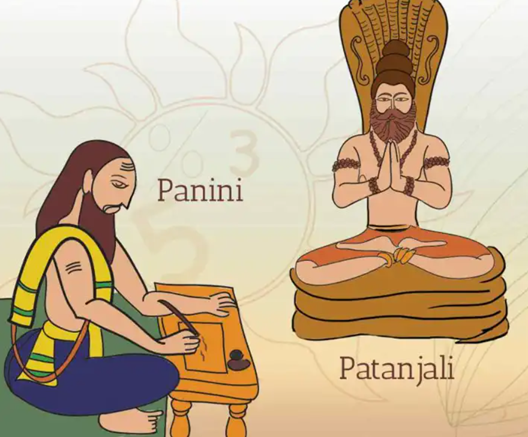
\includegraphics[width=0.3\linewidth,keepaspectratio]{images/patanjalipanini}
\end{center}


\tiny{(Ref: Sadhguru on Patanjali, Sushruta and Panini)}

\end{frame}



%%%%%%%%%%%%%%%%%%%%%%%%%%%%%%%%%%%%%%%%%%%%%%%%%%%%%%%%%%%
\begin{frame}[fragile]\frametitle{ योग सूत्र Yog Sutra}

	\begin{itemize}\item ``Yoga Sutra'': widely regarded as the authoritative text on `yoga'
	\item Collection Aphorisms, outlining the eight limbs of yoga.
	\item Sutras सूत्र (in Sanskrit) literally means a thread or string धागा that holds things together and more metaphorically refers to an aphorism	
	\item Guided by a single thread, a kite can glide and soar to amazing heights. 
	\item 	The Yoga Sutras of Patanjali are life’s threads, each one rich with knowledge, tools, and techniques. These sutras guide not only the mind but also one’s very being to its full potential. 
	\item 	Basically, Patanjali’s Yoga Sutras offer a systematic form of wisdom for attaining self-realization/enlightenment.
	\end{itemize}

\tiny{(Ref: Patanjali Yoga Sutra Dr Mrudula Chaudhari)}

\end{frame}


%%%%%%%%%%%%%%%%%%%%%%%%%%%%%%%%%%%%%%%%%%%%%%%%%%%%%%%%%%%
\begin{frame}[fragile]\frametitle{ योग सूत्र Yog Sutra}

	\begin{itemize}
	\item Minimum words, Unquestioned, Precise, essence, coherent eg. SthirSukhamAsan ( स्थिरसुखमासनम्| )
	\item Hard to understand by themselves so commentaries are needed.
	\item भाष्य commentaries starting with Vyas, are still going on (a living tradition)
	\item Vyasa's commentaries are highly regarded and have to be read along with Sutras.
	\end{itemize}

\tiny{(Ref: Patanjali Yoga Sutra Dr Mrudula Chaudhari)}

\end{frame}



%%%%%%%%%%%%%%%%%%%%%%%%%%%%%%%%%%%%%%%%%%%%%%%%%%%%%%%%%%%
\begin{frame}[fragile]\frametitle{Background}

	\begin{itemize}
	\item Patanjali Yog sutra emerged in the late Upanishad (उपनिषद) period
	\item Upanishads are earlier spiritual texts, but they are not systematic. They are mainly poetic expressions, metaphors some times confusing
	\item Examples: sometimes ब्रह्म साकार, sometimes ब्रह्म निराकार; जगन मिथ्या, जगन माया, जगन सत्य; आत्मन merges into ब्रह्मन्, etc). 
	\item Need to systematize.
	\end{itemize}

\tiny{(Ref: The Yoga Sutras of Patanjali | Prof. Edwin Bryant)}

\end{frame}

%%%%%%%%%%%%%%%%%%%%%%%%%%%%%%%%%%%%%%%%%%%%%%%%%%%%%%%%%%%
\begin{frame}[fragile]\frametitle{Systematization}

	\begin{itemize}
	\item Badarayana बादरायण codified unstructured Upanishad  उपनिषद texts.
	\item You get a few references to Yog in the Upanishads.
	\item Mentioned as techniques to attain ataman/brahman (आत्मन/ब्रह्मन्)
	\item Patanjali comes, systematizes and writes Yog Sutra (अथ अनुशाशन, continuing teachings of yog)
	\end{itemize}

\tiny{(Ref: The Yoga Sutras of Patanjali | Prof. Edwin Bryant)}

\end{frame}

%%%%%%%%%%%%%%%%%%%%%%%%%%%%%%%%%%%%%%%%%%%%%%%%%%%%%%%%%%%
\begin{frame}[fragile]\frametitle{Structure}

	\begin{itemize}
	\item Yogsutra has been divided into 4 chapters. `paad` (पाद) means foot, or quarter, as used while saying watch-timings (स+पाद, plus quarter). As there are 4 parts, each is called as a quarter.
	\item Total 195 verses/aphorisms
	\item Division:
		\begin{itemize}
		\item Samadhipad समाधिपाद 51
		\item Sadhanpad साधनपाद 55
		\item Vibhutipad विभूतिपाद 55
		\item Kaivalyapad कैवल्यपाद 34
		\end{itemize}	
	\end{itemize}

\tiny{(Ref: पातंजल योग सूत्र | Yog Darshan - Yoga And Ayurveda Science Youtube channel)}

\end{frame}

%%%%%%%%%%%%%%%%%%%%%%%%%%%%%%%%%%%%%%%%%%%%%%%%%%%%%%%%%%%
\begin{frame}[fragile]\frametitle{Contents}

Different Yogic methods for different types of people.

Types of people (prakruti प्रकृति ) in the world:

	\begin{itemize}
	\item High (uttam उत्तम ) : Already in almost pure mental state. Get success with very less efforts (sadhana !!!) 
	\item Medium (madhyam मध्यम )
	\item Low (adham अधम): Least pure mental state. Need vigorous discipline
	\end{itemize}
	
\tiny{(Ref: पातंजल योग सूत्र | Yog Darshan - Yoga And Ayurveda Science Youtube channel)}

\end{frame}

%%%%%%%%%%%%%%%%%%%%%%%%%%%%%%%%%%%%%%%%%%%%%%%%%%%%%%%%%%%
\begin{frame}[fragile]\frametitle{Contents}

Methods to attain yogic state based on type:


	\begin{itemize}
	\item Samadhipad समाधिपाद : , for uttam prakrti people, along with study (abhyas अभ्यास) and renunciation (vairagya वैराग्य)
	\item Sadhanpad साधनपाद : for adham prakriti people. Ashtang yog to get rid off miseries in life.
	\item Vibhutipad विभूतिपाद : After doing sadhana (dharana धारणा, dhyaan ध्यान, samadhi समाधि), one can get certain powers (siddhi सिद्धि, vibhuti विभूति). Recommends not get enamored by these powers.
	\item Kaivalyapad कैवल्यपाद : State of self detachment (moksh मोक्ष, mukti मुक्ति)
	\end{itemize}	

\tiny{(Ref: पातंजल योग सूत्र | Yog Darshan - Yoga And Ayurveda Science Youtube channel)}

\end{frame}


%%%%%%%%%%%%%%%%%%%%%%%%%%%%%%%%%%%%%%%%%%%%%%%%%%%%%%%%%%%
\begin{frame}[fragile]\frametitle{Contents}
	\begin{itemize}
	\item Yog Sutra is a practice text, and not a knowledge text.
	\item The Knowledge part is covered in Sankhya darshan (साङ्ख्य दर्शन)
	\item It is assumed that you have gone through the knowledge texts before.
	\item Gita's yoga definition is ACTION oriented, whereas Patanjali definition is IN-ACTION oriented.
	\end{itemize}

\tiny{(Ref: The Yoga Sutras of Patanjali | Prof. Edwin Bryant)}

\end{frame}

%%%%%%%%%%%%%%%%%%%%%%%%%%%%%%%%%%%%%%%%%%%%%%%%%%%%%%%%%%%
\begin{frame}[fragile]\frametitle{Primary References}
	\begin{itemize}
	\item On many slides you will find info with interpretations from different folks. They are from  site Yoga Sutra Study https://yogasutrastudy.info/
		\begin{itemize}
		\item [HA]: Hariharananda Aranya
		\item [IT]: I. K. Taimni
		\item [VH]: Vyasa Houston
		\item [BM]: Barbara Miller
		\item [SS]: Swami Satchidananda
		\item [SP]: Swami Prabhavananda
		\item [SV]: Swami Vivekananda
		\end{itemize}	
	\item Also, many slides will have Samskrit vigraha and [untagged] meaning, that's mainly from https://patanjaliyogasutra.in/
	\end{itemize}

Highly indebted for making such valuable information open.

\end{frame}

%%%%%%%%%%%%%%%%%%%%%%%%%%%%%%%%%%%%%%%%%%%%%%%%%%%%%%%%%%%
\begin{frame}[fragile]\frametitle{Commentaries}
    
    \begin{itemize}
        \item \textbf{Ved Vyasa}
        \begin{itemize}
            \item Authored the first and most authoritative commentary, known as the Vyasa Bhashya.
            \item Provides extensive explanations of the sutras, laying the foundation for subsequent interpretations.
            \item Emphasizes the philosophical underpinnings and the practical aspects of Yoga.
        \end{itemize}
        
        \item \textbf{Raja Bhoja}
        \begin{itemize}
            \item Composed the Bhoja Vritti, a detailed and insightful commentary.
            \item Focuses on the integration of Yoga with other philosophical systems.
            \item Highlights the historical and cultural context of the sutras.
        \end{itemize}
        
        \item \textbf{Adi Shankara}
        \begin{itemize}
            \item Though primarily known for Advaita Vedanta, he also provided commentary on Yogasutra.
            \item Aligns the principles of Yoga with the non-dualistic approach of Advaita Vedanta.
            \item Emphasizes the unity of Atman and Brahman in the practice of Yoga.
        \end{itemize}
        
        \item \textbf{Swami Vivekananda}
        \begin{itemize}
            \item Modern interpreter who made the Yogasutra accessible to a global audience.
            \item His commentary in "Raja Yoga" simplifies complex concepts for contemporary readers.
            \item Emphasizes practical application and the psychological aspects of Yoga.
        \end{itemize}
    \end{itemize}
    
\end{frame}


%%%%%%%%%%%%%%%%%%%%%%%%%%%%%%%%%%%%%%%%%%%%%%%%%%%%%%%%%%%
\begin{frame}[fragile]\frametitle{Ref Card}

\begin{center}
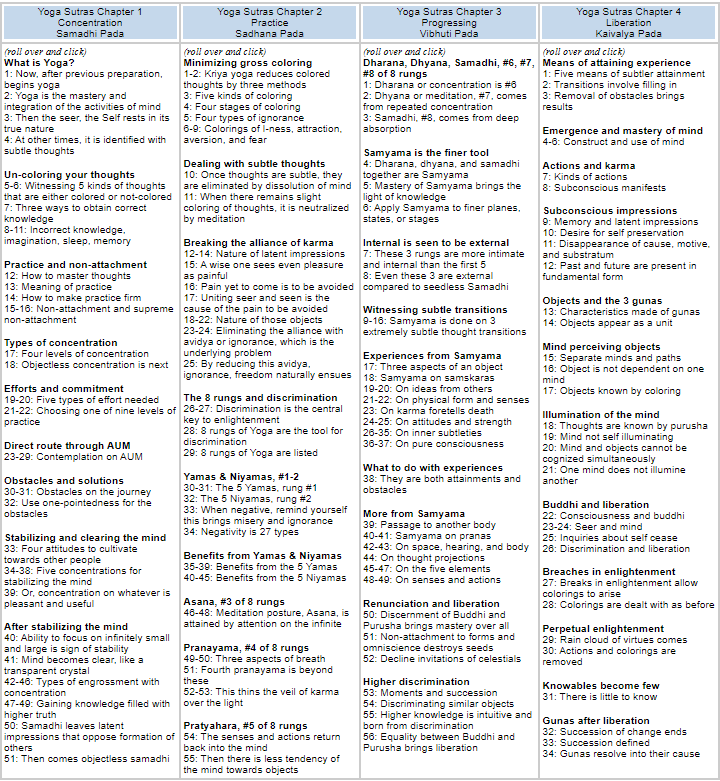
\includegraphics[width=0.6\linewidth,keepaspectratio]{SwamiJ_YogasutraCard}

\end{center}

  
  \tiny{(Ref: Yoga Sutras of Patanjali - Raja Yoga - Ashtanga Yoga - Swami J/Rama)}

\end{frame}


%%%%%%%%%%%%%%%%%%%%%%%%%%%%%%%%%%%%%%%%%%%%%%%%%%%%%%%%%%%
\begin{frame}[fragile]\frametitle{What are the Yoga Sutras?}

\begin{itemize}
\item Succinctly outlines art and science of Yoga meditation for Self-Realization
\item Systematically encountering and transcending levels of false identity in mind
\item Patanjali codified and compiled ancient practices in organized, terse way
\item Not a new system, but summarization of ancient practices
\item Thought to be as old as 400 BCE
\item Archaeological evidence suggests methods described were practiced as early as 3000 BCE
\item Oral tradition suggests even longer period
\item Process of examining and transcending gross and subtle levels of false identity
\item Until jewel of true Self shines through
\item Extremely organized and terse summarization of ancient practices
\end{itemize}

\begin{center}
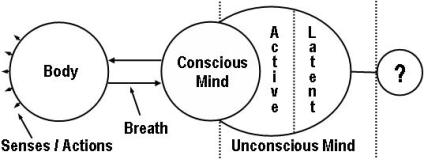
\includegraphics[width=0.4\linewidth,keepaspectratio]{yogaswamij1}

\end{center}

  
  \tiny{(Ref: Yoga Sutras of Patanjali - Raja Yoga - Ashtanga Yoga - Swami J/Rama)}

\end{frame}

%%%%%%%%%%%%%%%%%%%%%%%%%%%%%%%%%%%%%%%%%%%%%%%%%%%%%%%%%%%
\begin{frame}[fragile]\frametitle{Yoga means union \& sutra means thread}

\begin{itemize}
\item Yoga means union of parts of ourselves, never divided
\item Literally means to yoke, join, from the root "yuj"
\item Absorption in state of samadhi (union, enlightenment)
\item Sutra means thread, threads weave tapestry of insight and experience
\item Some say Sutras (plural) - each thread forms complete tapestry
\item Others say Sutra (singular) - one consistent thread through text
\item Both views provide useful perspective on process described
\item Union of parts refers to uniting different aspects of self
\item Never divided in first place, just perception of division
\item Direct experience and insight into true nature of reality
\end{itemize}

  
  \tiny{(Ref: Yoga Sutras of Patanjali - Raja Yoga - Ashtanga Yoga - Swami J/Rama)}

\end{frame}

%%%%%%%%%%%%%%%%%%%%%%%%%%%%%%%%%%%%%%%%%%%%%%%%%%%%%%%%%%%
\begin{frame}[fragile]\frametitle{Why Read the Yoga Sutras?}


\begin{center}
{\Large ``If you are on any path where you want to be happy, to be free of suffering, and understand the mind and consciousness, the Sutras are a must-read.''} – Edwin Bryant, Professor at Rutgers, PhD from Columbia
\end{center}

  

\end{frame}

%%%%%%%%%%%%%%%%%%%%%%%%%%%%%%%%%%%%%%%%%%%%%%%%%%%%%%%%%%%
\begin{frame}[fragile]\frametitle{Learning Path}

\begin{center}
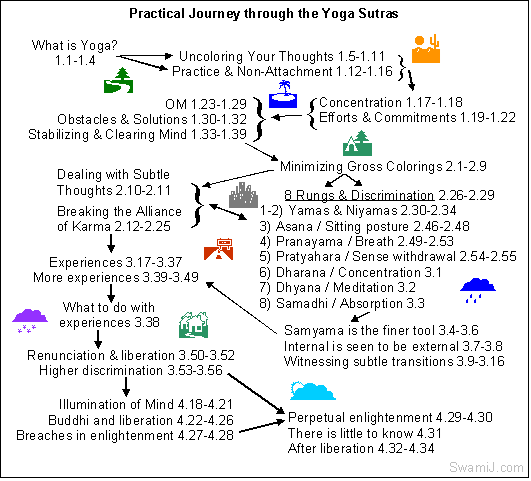
\includegraphics[width=0.6\linewidth,keepaspectratio]{SwamiJ_LearningPath}

\end{center}

  
  \tiny{(Ref: Yoga Sutras of Patanjali - Raja Yoga - Ashtanga Yoga - Swami J/Rama)}

\end{frame}


%%%%%%%%%%%%%%%%%%%%%%%%%%%%%%%%%%%%%%%%%%%%%%%%%%%%%%%%%%%
\begin{frame}[fragile]\frametitle{Other Names for Yoga}
\begin{itemize}
\item Raja Yoga (Royal Yoga)
\item Kriya Yoga (drawing on use of word 'Kriya' from Chapter 2)
\item Ashtanga Yoga (Eight-fold path of Yoga)
\item Includes yamas, niyamas, asana, pranayama, pratyahara, dharana, dhyana, samadhi
\item Begins with Sutra 28 of Chapter 2 (2.28)
\item Not referring to popularized physical yoga using same name
\item Ashtanga Yoga (Ashta = eight; anga = rungs)
\item Yamas (restraints), Niyamas (observances)
\item Asana (postures), Pranayama (breath control)
\item Pratyahara (withdrawal of senses), Dharana (concentration)
\item Dhyana (meditation), Samadhi (absorption, enlightenment)
\end{itemize}
  
  \tiny{(Ref: Yoga Sutras of Patanjali - Raja Yoga - Ashtanga Yoga - Swami J/Rama)}

\end{frame}


%%%%%%%%%%%%%%%%%%%%%%%%%%%%%%%%%%%%%%%%%%%%%%%%%%%%%%%%%%%
\begin{frame}[fragile]\frametitle{Yoga Sutras - Chapter 1: Concentration Samadhi Pada}
\begin{itemize}
\item What is Yoga? (1.1-1.4)
\item Un-Coloring Your Thoughts (1.5-1.11)
\item Practice and Non-Attachment (1.12-1.16)
\item Types of Concentration (1.17-1.18)
\item Efforts and Commitment (1.19-1.22)
\item Direct Route Through AUM (1.23-1.29)
\item Obstacles and Solutions (1.30-1.32)
\item Stabilizing and Clearing the Mind (1.33-1.39)
\item After Stabilizing the Mind (1.40-1.51)
\end{itemize}
\end{frame}

%%%%%%%%%%%%%%%%%%%%%%%%%%%%%%%%%%%%%%%%%%%%%%%%%%%%%%%%%%%
\begin{frame}[fragile]\frametitle{What is Yoga? (1.1-1.4)}
\begin{itemize}
\item 1.1: Now, after previous preparation, begins yoga
\item 1.2: Yoga is mastery and integration of mind activities
\item 1.3: Then the seer, the Self rests in true nature  
\item 1.4: At other times, identified with subtle thoughts
\end{itemize}
\end{frame}

%%%%%%%%%%%%%%%%%%%%%%%%%%%%%%%%%%%%%%%%%%%%%%%%%%%%%%%%%%%
\begin{frame}[fragile]\frametitle{Un-Coloring Your Thoughts (1.5-1.11)}
\begin{itemize}
\item 1.5-1.6: Witnessing 5 kinds of thoughts, colored or not
\item 1.7: Three ways to obtain correct knowledge
\item 1.8-1.11: Incorrect knowledge, imagination, sleep, memory
\end{itemize}
\end{frame}

%%%%%%%%%%%%%%%%%%%%%%%%%%%%%%%%%%%%%%%%%%%%%%%%%%%%%%%%%%%
\begin{frame}[fragile]\frametitle{Practice and Non-Attachment (1.12-1.16)}
\begin{itemize}
\item 1.12: How to master thoughts
\item 1.13: Meaning of practice
\item 1.14: How to make practice firm
\item 1.15-1.16: Non-attachment and supreme non-attachment
\end{itemize}
\end{frame}

%%%%%%%%%%%%%%%%%%%%%%%%%%%%%%%%%%%%%%%%%%%%%%%%%%%%%%%%%%%
\begin{frame}[fragile]\frametitle{Types of Concentration (1.17-1.18)}
\begin{itemize}
\item 1.17: Four levels of concentration
\item 1.18: Objectless concentration is next
\end{itemize}
\end{frame}

%%%%%%%%%%%%%%%%%%%%%%%%%%%%%%%%%%%%%%%%%%%%%%%%%%%%%%%%%%%
\begin{frame}[fragile]\frametitle{Efforts and Commitment (1.19-1.22)}
\begin{itemize}
\item 1.19-1.20: Five types of effort needed
\item 1.21-1.22: Choosing one of nine levels of practice
\end{itemize}
\end{frame}

%%%%%%%%%%%%%%%%%%%%%%%%%%%%%%%%%%%%%%%%%%%%%%%%%%%%%%%%%%%
\begin{frame}[fragile]\frametitle{Direct Route Through AUM (1.23-1.29)}
\begin{itemize}
\item 1.23-1.29: Contemplation on AUM
\end{itemize}
\end{frame}

%%%%%%%%%%%%%%%%%%%%%%%%%%%%%%%%%%%%%%%%%%%%%%%%%%%%%%%%%%%
\begin{frame}[fragile]\frametitle{Obstacles and Solutions (1.30-1.32)}
\begin{itemize}
\item 1.30-1.31: Obstacles on the journey
\item 1.32: Use one-pointedness for obstacles
\end{itemize}
\end{frame}

%%%%%%%%%%%%%%%%%%%%%%%%%%%%%%%%%%%%%%%%%%%%%%%%%%%%%%%%%%%
\begin{frame}[fragile]\frametitle{Stabilizing and Clearing the Mind (1.33-1.39)}
\begin{itemize}
\item 1.33: Four attitudes towards others  
\item 1.34-1.38: Five concentrations for stabilizing mind
\item 1.39: Or, concentrate on what is pleasant and useful
\end{itemize}
\end{frame}

%%%%%%%%%%%%%%%%%%%%%%%%%%%%%%%%%%%%%%%%%%%%%%%%%%%%%%%%%%%
\begin{frame}[fragile]\frametitle{After Stabilizing the Mind (1.40-1.51)}
\begin{itemize}  
\item 1.40: Ability to focus on infinitely small/large 
\item 1.41: Mind becomes clear crystal
\item 1.42-1.46: Types of engrossment in concentration
\item 1.47-1.49: Gaining higher truth knowledge
\item 1.50: Samadhi leaves opposing latent impressions
\item 1.51: Then comes objectless samadhi
\end{itemize}
\end{frame}

%%%%%%%%%%%%%%%%%%%%%%%%%%%%%%%%%%%%%%%%%%%%%%%%%%%%%%%%%%%
\begin{frame}[fragile]\frametitle{Yoga Sutras - Chapter 2: Practice Sadhana Pada}
\begin{itemize}
\item Minimizing Gross Coloring (2.1-2.9)
\item Dealing with Subtle Thoughts (2.10-2.11)  
\item Breaking the Alliance of Karma (2.12-2.25)
\item The 8 Rungs and Discrimination (2.26-2.29)
\item Yamas \& Niyamas, \#1-2 (2.30-2.34)
\item Benefits from Yamas \&Niyamas (2.35-2.45)
\item Asana, \#3 of 8 Rungs (2.46-2.48)
\item Pranayama, \#4 of 8 Rungs (2.49-2.53)
\item Pratyahara, \#5 of 8 Rungs (2.54-2.55)
\end{itemize}
\end{frame}

%%%%%%%%%%%%%%%%%%%%%%%%%%%%%%%%%%%%%%%%%%%%%%%%%%%%%%%%%%%
\begin{frame}[fragile]\frametitle{Minimizing Gross Coloring (2.1-2.9)}
\begin{itemize}
\item 2.1-2.2: Kriya yoga reduces colored thoughts
\item 2.3: Five kinds of coloring
\item 2.4: Four stages of coloring 
\item 2.5: Four types of ignorance
\item 2.6-2.9: Colorings of I-ness, attraction, aversion, fear
\end{itemize}
\end{frame}

%%%%%%%%%%%%%%%%%%%%%%%%%%%%%%%%%%%%%%%%%%%%%%%%%%%%%%%%%%%
\begin{frame}[fragile]\frametitle{Dealing with Subtle Thoughts (2.10-2.11)}
\begin{itemize}
\item 2.10: Subtle thoughts eliminated by mind dissolution
\item 2.11: Slight coloring neutralized by meditation  
\end{itemize}
\end{frame}

%%%%%%%%%%%%%%%%%%%%%%%%%%%%%%%%%%%%%%%%%%%%%%%%%%%%%%%%%%%
\begin{frame}[fragile]\frametitle{Breaking the Alliance of Karma (2.12-2.25)}
\begin{itemize}
\item 2.12-2.14: Nature of latent impressions
\item 2.15: The wise see even pleasure as painful
\item 2.16: Pain yet to come is to be avoided
\item 2.17: Cause of pain is uniting seer and seen
\item 2.18-2.22: Nature of those objects
\item 2.23-2.24: Eliminating alliance with ignorance
\item 2.25: Reducing ignorance leads to freedom
\end{itemize}  
\end{frame}

%%%%%%%%%%%%%%%%%%%%%%%%%%%%%%%%%%%%%%%%%%%%%%%%%%%%%%%%%%%
\begin{frame}[fragile]\frametitle{The 8 Rungs and Discrimination (2.26-2.29)}
\begin{itemize}
\item 2.26-2.27: Discrimination is key to enlightenment
\item 2.28: 8 rungs of Yoga are the tool  
\item 2.29: 8 rungs are listed
\end{itemize}
\end{frame}

%%%%%%%%%%%%%%%%%%%%%%%%%%%%%%%%%%%%%%%%%%%%%%%%%%%%%%%%%%%
\begin{frame}[fragile]\frametitle{Yamas \& Niyamas, \#1-2 (2.30-2.34)}
\begin{itemize}
\item 2.30-2.31: The 5 Yamas, rung \#1
\item 2.32: The 5 Niyamas, rung \#2
\item 2.33: Remind yourself negativity brings misery
\item 2.34: 27 types of negativity
\end{itemize}
\end{frame}

%%%%%%%%%%%%%%%%%%%%%%%%%%%%%%%%%%%%%%%%%%%%%%%%%%%%%%%%%%%
\begin{frame}[fragile]\frametitle{Benefits from Yamas \&Niyamas (2.35-2.45)}
\begin{itemize}
\item 2.35-2.39: Benefits from the 5 Yamas
\item 2.40-2.45: Benefits from the 5 Niyamas
\end{itemize}
\end{frame}

%%%%%%%%%%%%%%%%%%%%%%%%%%%%%%%%%%%%%%%%%%%%%%%%%%%%%%%%%%%
\begin{frame}[fragile]\frametitle{Asana, \#3 of 8 Rungs (2.46-2.48)}
\begin{itemize}
\item 2.46-2.48: Meditation posture by infinity attention
\end{itemize}
\end{frame}

%%%%%%%%%%%%%%%%%%%%%%%%%%%%%%%%%%%%%%%%%%%%%%%%%%%%%%%%%%%
\begin{frame}[fragile]\frametitle{Pranayama, \#4 of 8 Rungs (2.49-2.53)} 
\begin{itemize}
\item 2.49-2.50: Three aspects of breath
\item 2.51: Fourth pranayama beyond these
\item 2.52-2.53: Thins veil of karma over the light
\end{itemize}
\end{frame}

%%%%%%%%%%%%%%%%%%%%%%%%%%%%%%%%%%%%%%%%%%%%%%%%%%%%%%%%%%%
\begin{frame}[fragile]\frametitle{Pratyahara, \#5 of 8 Rungs (2.54-2.55)}
\begin{itemize}
\item 2.54: Senses return back into the mind
\item 2.55: Less tendency of mind towards objects 
\end{itemize}
\end{frame}

%%%%%%%%%%%%%%%%%%%%%%%%%%%%%%%%%%%%%%%%%%%%%%%%%%%%%%%%%%%
\begin{frame}[fragile]\frametitle{Yoga Sutras - Chapter 3: Progressing Vibhuti Pada}
\begin{itemize}
\item Dharana, Dhyana, Samadhi (\#6, \#7, \#8) (3.1-3.3)
\item Samyama is the Finer Tool (3.4-3.6)
\item Internal is Seen to be External (3.7-3.8)
\item Witnessing Subtle Transitions (3.9-3.16)
\item Experiences from Samyama (3.17-3.37)
\item What to Do with Experiences (3.38)
\item More from Samyama (3.39-3.49)
\item Renunciation and Liberation (3.50-3.52)
\item Higher Discrimination (3.53-3.56)
\end{itemize}
\end{frame}

%%%%%%%%%%%%%%%%%%%%%%%%%%%%%%%%%%%%%%%%%%%%%%%%%%%%%%%%%%%
\begin{frame}[fragile]\frametitle{Dharana, Dhyana, Samadhi (\#6, \#7, \#8) (3.1-3.3)}
\begin{itemize}
\item 3.1: Dharana or concentration is \#6
\item 3.2: Dhyana or meditation (\#7) from repeated dharana
\item 3.3: Samadhi (\#8) from deep absorption
\end{itemize}
\end{frame}

%%%%%%%%%%%%%%%%%%%%%%%%%%%%%%%%%%%%%%%%%%%%%%%%%%%%%%%%%%%
\begin{frame}[fragile]\frametitle{Samyama is the Finer Tool (3.4-3.6)}
\begin{itemize}
\item 3.4: Dharana, dhyana, samadhi together are Samyama
\item 3.5: Mastery of Samyama brings light of knowledge
\item 3.6: Apply Samyama to finer planes, states, stages
\end{itemize}
\end{frame}

%%%%%%%%%%%%%%%%%%%%%%%%%%%%%%%%%%%%%%%%%%%%%%%%%%%%%%%%%%%
\begin{frame}[fragile]\frametitle{Internal is Seen to be External (3.7-3.8)}
\begin{itemize}
\item 3.7: These 3 rungs more intimate, internal than first 5
\item 3.8: Even these 3 external compared to seedless Samadhi
\end{itemize}
\end{frame}

%%%%%%%%%%%%%%%%%%%%%%%%%%%%%%%%%%%%%%%%%%%%%%%%%%%%%%%%%%%
\begin{frame}[fragile]\frametitle{Witnessing Subtle Transitions (3.9-3.16)}
\begin{itemize}
\item 3.9-3.16: Samyama on 3 extremely subtle thought transitions
\end{itemize}
\end{frame}

%%%%%%%%%%%%%%%%%%%%%%%%%%%%%%%%%%%%%%%%%%%%%%%%%%%%%%%%%%%
\begin{frame}[fragile]\frametitle{Experiences from Samyama (3.17-3.37)}
\begin{itemize}
\item 3.17: Three aspects of an object
\item 3.18: Samyama on samskaras
\item 3.19-3.20: On ideas from others
\item 3.21-3.22: On physical form and senses
\item 3.23: On karma foretells death
\item 3.24-3.25: On attitudes and strength
\item 3.26-3.35: On inner subtleties
\item 3.36-3.37: On pure consciousness
\end{itemize}
\end{frame}

%%%%%%%%%%%%%%%%%%%%%%%%%%%%%%%%%%%%%%%%%%%%%%%%%%%%%%%%%%%
\begin{frame}[fragile]\frametitle{What to Do with Experiences (3.38)}
\begin{itemize}  
\item 3.38: Experiences are attainments and obstacles
\end{itemize}
\end{frame}

%%%%%%%%%%%%%%%%%%%%%%%%%%%%%%%%%%%%%%%%%%%%%%%%%%%%%%%%%%%
\begin{frame}[fragile]\frametitle{More from Samyama (3.39-3.49)}
\begin{itemize}
\item 3.39: Passage to another body
\item 3.40-3.41: On pranas
\item 3.42-3.43: On space, hearing, body
\item 3.44: On thought projections
\item 3.45-3.47: On five elements
\item 3.48-3.49: On senses and actions
\end{itemize}
\end{frame}

%%%%%%%%%%%%%%%%%%%%%%%%%%%%%%%%%%%%%%%%%%%%%%%%%%%%%%%%%%%
\begin{frame}[fragile]\frametitle{Renunciation and Liberation (3.50-3.52)}
\begin{itemize}
\item 3.50: Discerning Buddhi and Purusha brings mastery
\item 3.51: Non-attachment destroys seeds, omniscience
\item 3.52: Decline celestial invitations  
\end{itemize}
\end{frame}

%%%%%%%%%%%%%%%%%%%%%%%%%%%%%%%%%%%%%%%%%%%%%%%%%%%%%%%%%%%
\begin{frame}[fragile]\frametitle{Higher Discrimination (3.53-3.56)}
\begin{itemize}
\item 3.53: Moments and succession
\item 3.54: Discriminating similar objects
\item 3.55: Higher intuitive knowledge from discrimination
\item 3.56: Equality of Buddhi and Purusha brings liberation
\end{itemize}
\end{frame}

%%%%%%%%%%%%%%%%%%%%%%%%%%%%%%%%%%%%%%%%%%%%%%%%%%%%%%%%%%%
\begin{frame}[fragile]\frametitle{Yoga Sutras - Chapter 4: Liberation Kaivalya Pada}
\begin{itemize}
\item Means of Attaining Experience (4.1-4.3)
\item Emergence and Mastery of Mind (4.4-4.6)
\item Actions and Karma (4.7-4.8)
\item Subconscious Impressions (4.9-4.12)
\item Objects and the 3 Gunas (4.13-4.14)
\item Mind Perceiving Objects (4.15-4.17)
\item Illumination of the Mind (4.18-4.21)
\item Buddhi and Liberation (4.22-4.26)
\item Breaches in Enlightenment (4.27-4.28)
\item Perpetual Enlightenment (4.29-4.30)
\item Knowables Become Few (4.31)
\item Gunas After Liberation (4.32-4.34)
\end{itemize}
\end{frame}

%%%%%%%%%%%%%%%%%%%%%%%%%%%%%%%%%%%%%%%%%%%%%%%%%%%%%%%%%%%
\begin{frame}[fragile]\frametitle{Means of Attaining Experience (4.1-4.3)}
\begin{itemize}
\item 4.1: Five means of subtler attainment
\item 4.2: Transitions involve filling in
\item 4.3: Removal of obstacles brings results
\end{itemize}
\end{frame}

%%%%%%%%%%%%%%%%%%%%%%%%%%%%%%%%%%%%%%%%%%%%%%%%%%%%%%%%%%%
\begin{frame}[fragile]\frametitle{Emergence and Mastery of Mind (4.4-4.6)}
\begin{itemize}
\item 4.4-4.6: Construct and use of mind
\end{itemize}
\end{frame}

%%%%%%%%%%%%%%%%%%%%%%%%%%%%%%%%%%%%%%%%%%%%%%%%%%%%%%%%%%%
\begin{frame}[fragile]\frametitle{Actions and Karma (4.7-4.8)}
\begin{itemize}
\item 4.7: Kinds of actions
\item 4.8: Subconscious manifests
\end{itemize}
\end{frame}

%%%%%%%%%%%%%%%%%%%%%%%%%%%%%%%%%%%%%%%%%%%%%%%%%%%%%%%%%%%
\begin{frame}[fragile]\frametitle{Subconscious Impressions (4.9-4.12)}
\begin{itemize}
\item 4.9: Memory and latent impressions
\item 4.10: Desire for self preservation
\item 4.11: Disappearance of cause, motive, substratum
\item 4.12: Past and future are present fundamentally
\end{itemize}
\end{frame}

%%%%%%%%%%%%%%%%%%%%%%%%%%%%%%%%%%%%%%%%%%%%%%%%%%%%%%%%%%%
\begin{frame}[fragile]\frametitle{Objects and the 3 Gunas (4.13-4.14)}
\begin{itemize}
\item 4.13: Characteristics made of gunas
\item 4.14: Objects appear as a unit
\end{itemize}
\end{frame}

%%%%%%%%%%%%%%%%%%%%%%%%%%%%%%%%%%%%%%%%%%%%%%%%%%%%%%%%%%%
\begin{frame}[fragile]\frametitle{Mind Perceiving Objects (4.15-4.17)}
\begin{itemize}
\item 4.15: Separate minds and paths
\item 4.16: Object not dependent on one mind
\item 4.17: Objects known by coloring
\end{itemize}
\end{frame}

%%%%%%%%%%%%%%%%%%%%%%%%%%%%%%%%%%%%%%%%%%%%%%%%%%%%%%%%%%%
\begin{frame}[fragile]\frametitle{Illumination of the Mind (4.18-4.21)}
\begin{itemize}
\item 4.18: Thoughts known by purusha
\item 4.19: Mind not self illuminating
\item 4.20: Mind and objects can't be cognized together  
\item 4.21: One mind doesn't illumine another
\end{itemize}
\end{frame}

%%%%%%%%%%%%%%%%%%%%%%%%%%%%%%%%%%%%%%%%%%%%%%%%%%%%%%%%%%%
\begin{frame}[fragile]\frametitle{Buddhi and Liberation (4.22-4.26)}
\begin{itemize}
\item 4.22: Consciousness and buddhi
\item 4.23-4.24: Seer and mind
\item 4.25: Inquiries about self cease  
\item 4.26: Discrimination and liberation
\end{itemize}
\end{frame}

%%%%%%%%%%%%%%%%%%%%%%%%%%%%%%%%%%%%%%%%%%%%%%%%%%%%%%%%%%%
\begin{frame}[fragile]\frametitle{Breaches in Enlightenment (4.27-4.28)}
\begin{itemize}
\item 4.27: Breaks allow colorings to arise
\item 4.28: Colorings dealt with as before
\end{itemize}  
\end{frame}

%%%%%%%%%%%%%%%%%%%%%%%%%%%%%%%%%%%%%%%%%%%%%%%%%%%%%%%%%%%
\begin{frame}[fragile]\frametitle{Perpetual Enlightenment (4.29-4.30)}
\begin{itemize}
\item 4.29: Rain cloud of virtues comes 
\item 4.30: Actions and colorings removed
\end{itemize}
\end{frame}

%%%%%%%%%%%%%%%%%%%%%%%%%%%%%%%%%%%%%%%%%%%%%%%%%%%%%%%%%%%
\begin{frame}[fragile]\frametitle{Knowables Become Few (4.31)}
\begin{itemize}
\item 4.31: There is little to know
\end{itemize}
\end{frame}

%%%%%%%%%%%%%%%%%%%%%%%%%%%%%%%%%%%%%%%%%%%%%%%%%%%%%%%%%%%
\begin{frame}[fragile]\frametitle{Gunas After Liberation (4.32-4.34)} 
\begin{itemize}
\item 4.32: Succession of change ends
\item 4.33: Succession defined
\item 4.34: Gunas resolve into their cause
\end{itemize}
\end{frame}

